%!TEX root = ../tesis.tex
\chapter{Definici\'on del Problema}
\label{sec:problema}

El reconocimiento del habla es un área de investigación amplia y sus aplicaciones, que se han presentado
previamente, son diversas. Este capítulo presenta y describe el problema abordado en este trabajo
de investigación, su alcance y la motivación del mismo, de modo a establecer con claridad los límites
y el propósito del estudio realizado.

% introduccion

%!TEX root = ../tesis.tex
\section{Descripci\'on General}
\label{sec:problema-general}

El reconocimiento del habla (tambi\'en conocido como reconocimiento autom\'atico del habla) es el proceso
de convertir una se\~nal de voz en una secuencia de palabras, mediante un algoritmo implementado
como programa \mbox{computacional \cite{JaisalAReview2012}}.

Las interfaces mediante voz del usuario son sistemas computaciones especializados que permiten la
interacci\'on entre seres humanos y computadoras (otros sistemas computacionales) a trav\'es de
s{\'\i}ntesis y reconocimiento del habla. Estas interfaces presentan ciertas caracter{\'\i}sticas que las
distinguen de las interfaces visuales \cite{GabrielVoice2007}:

\begin{itemize}
	\item Transitoriedad: la voz desaparece tan pronto como se termina de pronunciar una oraci\'on,
	lo cual obliga a recordar lo que se dijo. Las interfaces visuales, por otro lado, son persistentes.
	\item Invisibilidad: la voz no es visible, lo cual hace dif{\'\i}cil indicar al usuario las opciones
	disponibles y los comandos necesarios para ejecutarlas. En las interfaces visuales los men\'ues
	cumplen esta funci\'on.
	\item Asimetr{\'\i}a: la voz puede producirse r\'apidamente, pero comprender lo que se escucha requiere
	m\'as tiempo. As{\'\i}, un usuario puede hablar m\'as r\'apido de lo que escribe con un teclado; sin embargo,
	al usuario le toma m\'as tiempo comprender lo que escucha que lo que lee.
\end{itemize}

Estas caracter{\'\i}sticas suponen un desaf{\'\i}o adicional al momento de dise\~nar interfaces mediante voz del
usuario. A\'un as{\'\i}, estas interfaces poseen un gran potencial en situaciones en las cuales la
combinaci\'on tradicional de teclado, rat\'on y monitor resulta problem\'atica \cite{NielsenVoice2003}:

\begin{itemize}
	\item Usuarios con discapacidades, las cuales les impiden manejar apropiadamente el rat\'on y/o
	el teclado o visualizar la informaci\'on en el monitor.
	\item Usuarios en situaciones de manos y vista ocupadas: como la conducci\'on de un veh{\'\i}culo o
	la reparaci\'on de equipamiento complejo.
	\item Usuarios sin acceso a un teclado o monitor: en este caso los usuarios podr{\'\i}an acceder
	a un sistema a trav\'es de un tel\'efono convencional.
\end{itemize}


%!TEX root = ../tesis.tex
\section{Alcance}
\label{sec:problema-especifico}

De modo a contrastar la pr\'actica con el conocimiento te\'orico adquirido en
el transcurso de este trabajo de investigaci\'on, se incluye el dise\~no e implementaci\'on de
una interfaz mediante voz del usuario para una aplicaci\'on como parte del mismo.

Para obtener conclusiones del proceso de dise\~no e implementaci\'on y de la posterior evaluaci\'on
de la interfaz, se consider\'o que la misma deb{\'\i}a ser de cierta complejidad. Esto es, la
aplicaci\'on implementada deb{\'\i}a cumplir con los siguientes requisitos:

\begin{itemize}
     \item Nivel de interacci\'on medio o alto entre el usuario y la aplicaci\'on.
     \item Lenguaje de tama\~no considerable.
     \item Comandos reconocidos de varias longitudes.
     \item Interacci\'on normalmente prolongada entre el usuario y la aplicaci\'on.
 \end{itemize} 

Cumpliendo con las condiciones anteriormente mencionadas, se decidi\'o dise\~nar e implementar 
una interfaz para un programa simple de composici\'on musical.
Se opt\'o por utilizar una interfaz multimodal, 
haciendo uso de soporte visual para minimizar el efecto de las limitaciones
relacionadas a la voz que se mencionaron previamente.

Las funcionalidades m{\'\i}nimas requeridas para el sistema se citan a continuaci\'on:
%Explicar mejor
\begin{itemize}
    \item El usuario puede crear m\'usica con la aplicaci\'on: esta es la funcionalidad de
    mayor importancia y el objetivo del sistema.
    \item El usuario puede seleccionar distintos instrumentos musicales: esto
    permite la combinaci\'on de los distintos instrumentos para la composici\'on de la m\'usica.
    \item El usuario puede configurar el volumen de cada instrumento musical: de
    modo a poder combinar los distintos instrumentos con distinta intensidad en el
    sonido.
    \item El usuario puede crear sonidos: un sonido es la unidad b\'asica para la
    creaci\'on de una m\'usica. B\'asicamente, se compone m\'usica mediante la combinaci\'on
    de sonidos.
    \item El usuario puede configurar el tono y la duraci\'on de los sonidos: de modo
    a permitir un gran n\'umero de combinaciones posibles para la composici\'on musical.
    \item El usuario puede reproducir, pausar y detener la m\'usica: de modo a poder
    escuchar y apreciar su obra.
    \item El usuario puede guardar la m\'usica que crea: de modo a poder escuchar
    su obra en reproductores de audio y compartirla.
\end{itemize}

Una vez definida la tem\'atica de la aplicaci\'on a implementar, llevar a la pr\'actica
los conocimientos adquiridos requiere definir ciertas cuestiones:

\begin{itemize}
    \item Definici\'on de Comandos: se refiere al proceso de definir el comando, o la secuencia de
    comandos, que se utilizar\'a para exponer cada funcionalidad prove{\'\i}da por el sistema.

    El lenguaje aceptado define la interacci\'on entre el usuario y la aplicaci\'on, y es de esperarse
    que resulte importante para la naturalidad de la misma y para la usabilidad del sistema en
    general.

    \item Herramientas a utilizar: existe un gran n\'umero de opciones disponibles
    para la implementaci\'on de una interfaz basada en voz del usuario.
    La selecci\'on de la herramienta tiene un gran impacto sobre el proceso de implementaci\'on
    y debe realizarse de acuerdo a las prioridades del caso.

    La clasificaci\'on y evaluaci\'on inclu{\'\i}da en el cap{\'\i}tulo anterior puede resultar de
    utilidad para tomar esta decisi\'on de manera informada y en base a criterios bien establecidos.

    \item Evaluaci\'on de la Aplicaci\'on: una evaluaci\'on de la aplicaci\'on implementada puede ayudar
    a identificar problemas y sugerir mejoras o nuevas funcionalidades. Adem\'as, en el caso particular
    de este trabajo, se espera obtener conclusiones acerca de las interfaces basadas en el reconocimiento
    del habla.

    Para realizar la evaluaci\'on deben establecerse varios puntos como: los objetivos, la metodolog{\'\i}a,
    los factores a tener en cuenta, las m\'etricas que se utilizar\'an, etc.

 \end{itemize} 
%!TEX root = ../tesis.tex
\section{Motivaci\'on}
\label{sec:motivacion}

La habilidad de producir y entender el lenguaje oral ha sido se\~nalada por los antrop\'ologos
como uno de los principales logros de nuestra especie. Varios investigadores coinciden
en considerar el lenguaje como un instinto, una adaptaci\'on biol\'ogica que nos permite
comunicar \mbox{informaci\'on \cite{GabrielVoice2007}}.

Habiendo establecido la importancia del habla, resulta natural pensar en formas de
interactuar con las computadoras a trav\'es de estas interfaces.

De acuerdo a los reportes de la renombrada consultora tecnol\'ogica Gartner, el reconocimiento
del habla alcanzara la  \emph{meseta de la productividad} en los pr\'oximos 2 a 5 a\~nos. Esto es,
se convertir\'a en una tecnolog{\'\i}a estable y cuyos beneficios est\'an ampliamente demostrados
y \mbox{aceptados \cite{Gartner2013}}.

\begin{figure}[ht]
\centering
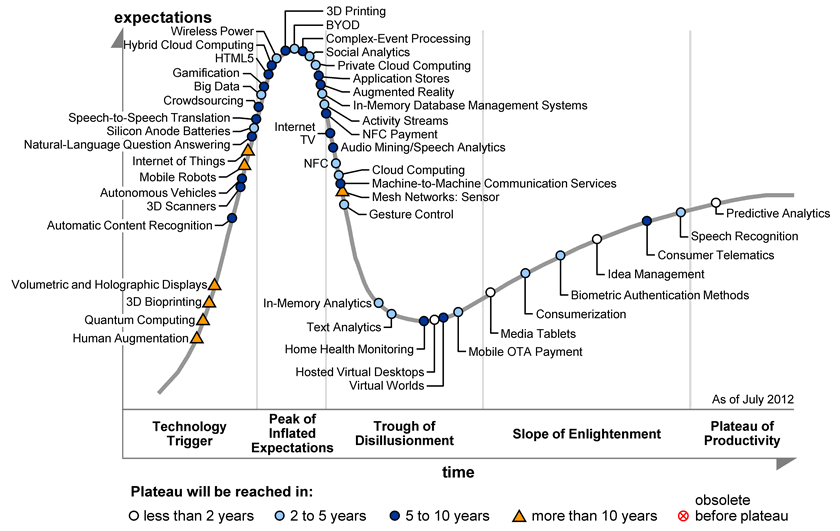
\includegraphics[width=0.8\linewidth]{./graphics/gartner.png}
\caption{Ciclo de Sobreexpectaci\'on de tecnolog{\'\i}as emergentes de \mbox{Gartner -- 2013 \cite{Gartner2013}.}}
\label{figure:gartner}
\end{figure}
%Figura Gartner

El dise\~no y la implementaci\'on de una interfaz mediante voz del usuario representa
una oportunidad, no solo para el estudio de esta \'area de investigaci\'on, sino para
demostrar la aplicabilidad del reconocimiento del habla a un problema real.

Habiendo mencionado previamente la potencial importancia del dominio de la aplicaci\'on
para una interfaz por voz del usuario, la elecci\'on de un programa de composici\'on musical
no pod{\'\i}a ser injustificada.
Existen investigaciones realizadas que relacionan a la m\'usica y el reconocimiento
del habla, en particular, orientadas al problema de recuperaci\'on de informaci\'on
\mbox{musical \cite{Goto2004Speech, Schuller2003Hybrid}}.
Sin embargo, resulta interesante explorar la utilizaci\'on del reconocimiento
del habla para la composici\'on musical. Este enfoque, en el cual un programa recibe comandos
sonoros y emite tambi\'en un resultado sonoro, podr{\'\i}a resultar incluso m\'as natural.

El programa de composici\'on musical controlado por voz es un medio para:

\begin{itemize}
	\item Explorar y experimentar con el reconocimiento del habla y las interfaces de usuario.
	\item Contrastar teor{\'\i}a y pr\'actica.
	\item Demostrar la factibilidad de la soluci\'on de un problema real utilizando el
	reconocimiento del habla.
\end{itemize}
